\chapterimage{../Pictures/iot.png}

\chapter{Repaso Express}
\vspace{160pt}

\section{Tomando los Requerimientos de la PuertaPerruna}

\begin{tcolorbox}[colback=gray!5!white,colframe=orange!60!gray,title=PuertaPerruna]
Los perros del siglo XXI también son independientes y el lema de esta empresa es "si se puede digitalizar/automatizar entonces digitalicémoslo/automaticémoslo". Como arquitecto de aplicaciones, apoyaremos en la prueba de concepto del sistema ciberfísico para la puerta perruna. La \textbf{PuertaPerruna} es un hardware de aproximadamente 40 cm de alto por 30 cm de ancho que se instala en la puerta de la casa y permite la salida y entrada del perro al patio a través de un sensor del ladrido. Si el sensor de ladrido reconoce el sonido del perro con el cual fue configurado, la puerta se activa y se abrirá o cerrará por un espacio de X segundos, teniendo un sensor de movimiento para evitar el cierre brusco y posible golpe al perro.
\end{tcolorbox}

\subsection{Requisitos Funcionales}
El sistema debe realizar las siguientes funciones:
\begin{itemize}
    \item RF1: \textbf{PuertaPerruna} deberá reconocer ladridos de perros registrados con una precisión superior al 98\%.
    \item RF2: \textbf{PuertaPerruna} deberá abrir la puerta.
    \item RF3: \textbf{PuertaPerruna} deberá cerrar la puerta.
    \item RF4: \textbf{PuertaPerruna} deberá determinar si es seguro cerrar.
    \item RF5: \textbf{PuertaPerruna} deberá saber siempre el estado de la puerta.
\end{itemize}

\subsection{Herramientas Utilizadas}
Para este caso utilizaremos las siguientes herramientas:
\begin{itemize}
    \item Python
    \item PlantUML
    \item VSCode
    \item Github
    \item copilot (opcional)
\end{itemize}

\begin{figure}[!h]
\centering
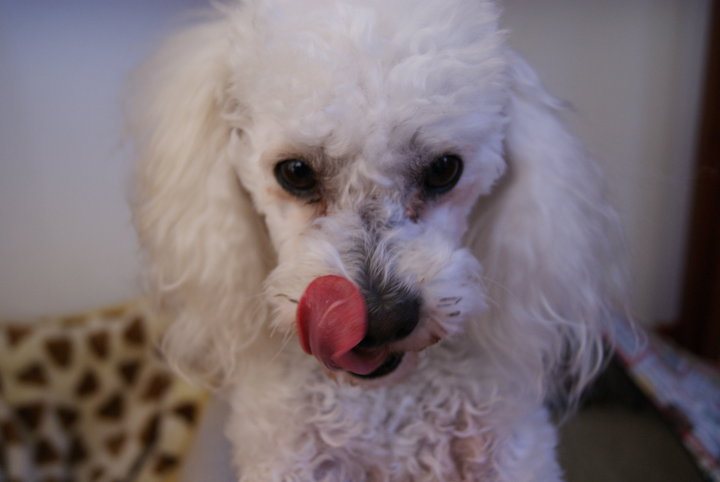
\includegraphics[scale=3]{Pictures/pompi.jpg}
\caption{Pompi, nuestro usuario de prueba para \textbf{PuertaPerruna} - un sistema que dará independencia a tus perros, y a ti, más horas de sueño.}
\label{fig:pompi}
\end{figure}

\subsection{Casos de Uso}
\subsubsection{Caso de Uso: Salir de Casa}
\begin{enumerate}
    \item \textbf{Actor}: El perro ladra dos veces frente a la puerta para poder salir.
    \item \textbf{Sistema}: El sensor de ladridos reconoce el ladrido del perro y envía la petición a la puerta para que se abra.
    \item \textbf{Sistema}: La puerta se abre.
    \item \textbf{Actor}: El perro sale.
    \item \textbf{Sistema}: La puerta espera X segundos y se cierra lentamente, volviéndose a abrir si detecta que aún hay movimiento y no es seguro cerrarse (reintentará cerrarse nuevamente luego de X segundos).
\end{enumerate}

\subsubsection{Caso de Uso: Entrar a Casa}
\begin{enumerate}
    \item \textbf{Actor}: El perro vuelve luego de hacer su negocio fuera de la casa y ladra para poder entrar.
    \item \textbf{Sistema}: El sensor de ladridos reconoce el ladrido del perro de la casa.
    \item \textbf{Sistema}: El sensor envía la petición a la puerta para que se abra.
    \item \textbf{Sistema}: La puerta se abre.
    \item \textbf{Actor}: El perro entra.
    \item \textbf{Sistema}: La puerta espera X segundos y se cierra lentamente, volviéndose a abrir si detecta que aún hay movimiento y no es seguro cerrarse (reintentará cerrarse nuevamente luego de X segundos).
\end{enumerate}

\begin{tcolorbox}[colback=gray!5!white,colframe=orange!60!gray,title=TODO]
Escribir a nivel de análisis el diagrama de secuencia para este flujo. Usar \url{https://pdf.plantuml.net/1.2021.1/PlantUML_Language_Reference_Guide_es.pdf}
\end{tcolorbox}

\subsection{Diagramas de Secuencia y Dominio}
\begin{tcolorbox}[colback=gray!5!white,colframe=orange!60!gray,title=Diagrama de Secuencia en PlantUML]
\begin{verbatim}
@startuml
actor Perro
participant "Sistema PuertaPerruna" as Sistema

Perro -> Sistema: Ladra para salir
Sistema -> Sistema: Detectar ladrido
Sistema -> Sistema: Abrir puerta
Sistema -> Perro: Puerta abierta
Perro -> Sistema: Sale
Sistema -> Sistema: Inicia temporizador para cerrar
Sistema -> Sistema: Detecta movimiento
Sistema -> Sistema: Cierra puerta si es seguro
@enduml
\end{verbatim}
\end{tcolorbox}

\begin{figure}[!h]
\centering
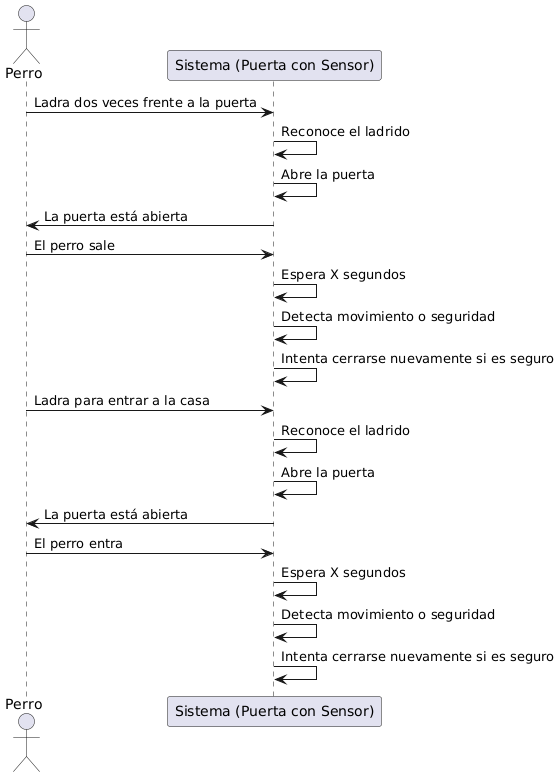
\includegraphics[scale=0.5]{Pictures/pp_analisis.png}
\caption{Diagrama a nivel de análisis.}
\label{fig:diag-sec}
\end{figure}

\begin{tcolorbox}[colback=gray!5!white,colframe=orange!60!gray,title=Modelo de Dominio en PlantUML]
\begin{verbatim}
@startuml
entity "Perro" as Perro {
    * nombre
    * raza
    * edad
}

entity "Puerta" as Puerta {
    * estado: {Abierta | Cerrada}
    * tiempo de cierre
}

entity "Sensor" as Sensor {
    * tipo: {Ladrido | Movimiento}
    * configurado: Boolean
}

Perro --|> Sensor : "Activa"
Sensor -- Puerta : "Controla"
@enduml
\end{verbatim}
\end{tcolorbox}

\begin{figure}[!h]
\centering
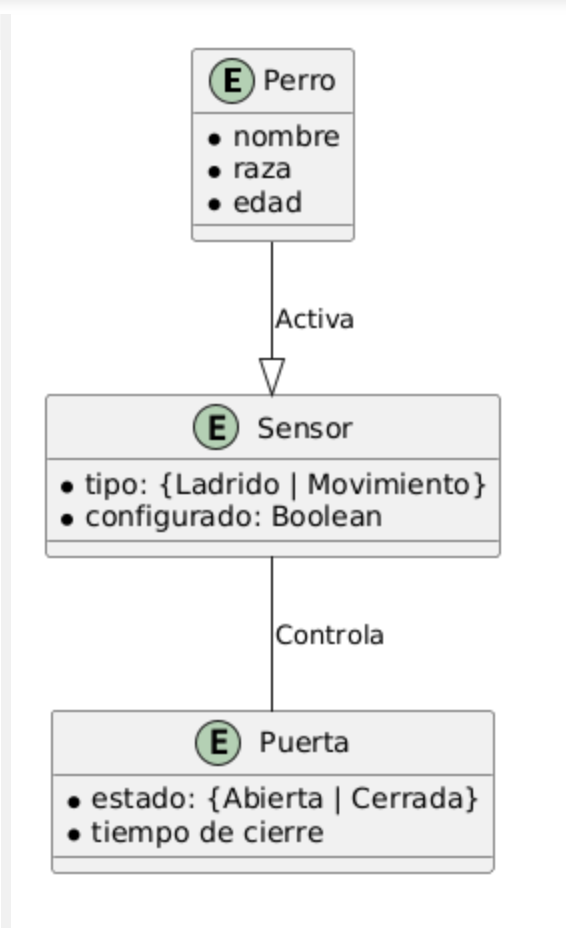
\includegraphics[scale=0.5]{Pictures/dominio.png}
\caption{Diagrama de dominio.}
\label{fig:diag-dom}
\end{figure}

\subsection{Diagrama de Estados}
El siguiente diagrama muestra los estados posibles de la \textbf{PuertaPerruna}:

\begin{tcolorbox}[colback=gray!5!white,colframe=orange!60!gray,title=Diagrama de Estados en PlantUML]
\begin{verbatim}
@startuml
[*] --> Cerrada
Cerrada --> Abierta: Detecta ladrido
Abierta --> Cerrada: Temporizador expira
Abierta --> Abierta: Detecta movimiento
Cerrada --> Cerrada: Sin eventos
@enduml
\end{verbatim}
\end{tcolorbox}

\begin{figure}[!h]
\centering
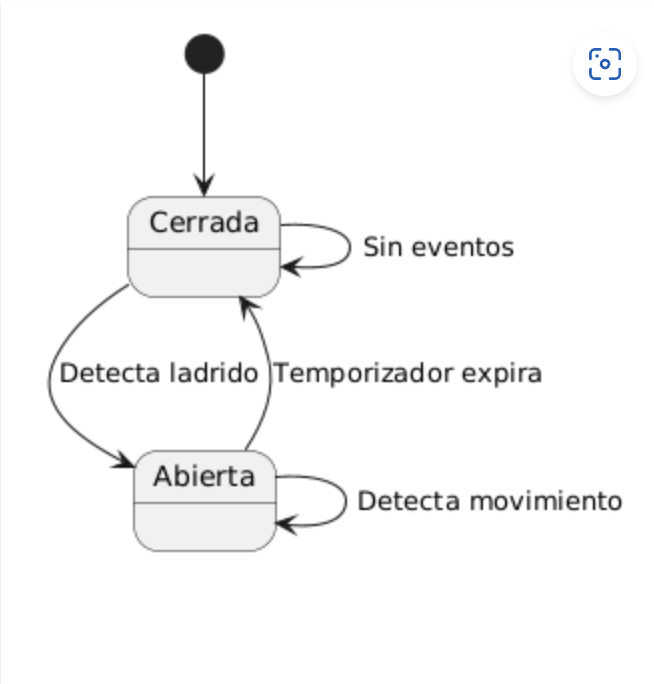
\includegraphics[scale=0.5]{Pictures/estados.png}
\caption{Diagrama de estado.}
\label{fig:diag-estado}
\end{figure}

\section*{Actividad: Preparación y Ejecución}

\subsection*{Parte 0: Tomar los Cursitos}
\begin{itemize}
    \item \url{https://github.com/skills/introduction-to-github}
    \item \url{https://github.com/skills/github-pages}
\end{itemize}

\subsection*{Parte 1: Creación del Repositorio}
Un integrante del equipo deberá:
\begin{enumerate}
    \item Crear un repositorio en GitHub con el nombre \texttt{PuertaPerruna}.
    \item Subir los archivos iniciales de código en Python.
    \item Compartir el enlace del repositorio con el equipo.
\end{enumerate}

\subsection*{Parte 2: Clonación y Ejecución}
Otro integrante deberá:
\begin{enumerate}
    \item Clonar el repositorio utilizando VSCode o el terminal con: \texttt{git clone <URL del repositorio>}.
    \item Ejecutar el archivo principal \texttt{simuladorBobby.py}.
    \item Comprobar el funcionamiento y realizar mejoras si es necesario.
\end{enumerate}

\subsection*{Parte 3: Adición de Casos de Prueba Unitaria usando IA Generativa}
\textbf{Objetivo:} Utilizar un chat de IA generativa para apoyar la creación de casos de prueba unitaria y ejecutarlos en Visual Studio Code (VSCode).

\textbf{Instrucciones:}
\begin{enumerate}
    \item \textbf{Preparación del Entorno:}
    \begin{itemize}
        \item Asegúrate de tener instalado VSCode y las extensiones necesarias para Python.
        \item Clona o descarga el código base proporcionado para la actividad.
    \end{itemize}
    
    \item \textbf{Uso de IA Generativa:}
    \begin{itemize}
        \item Utiliza un chat de IA generativa (como copilot integrado en VSCode) para obtener sugerencias sobre cómo escribir casos de prueba unitaria para el código base.
        \item Puedes formular preguntas específicas sobre cómo probar ciertas funciones o módulos del código.
    \end{itemize}
    
    \item \textbf{Escritura de Casos de Prueba:}
    \begin{itemize}
        \item Basándote en las sugerencias de la IA, escribe los casos de prueba unitaria en un archivo de prueba (por ejemplo, \texttt{test\_code.py}).
        \item Asegúrate de cubrir diferentes escenarios, incluyendo casos positivos y negativos.
    \end{itemize}
    
    \item \textbf{Ejecución de Pruebas:}
    \begin{itemize}
        \item Ejecuta los casos de prueba en VSCode utilizando una herramienta de pruebas como \texttt{unittest} o \texttt{pytest}.
        \item Verifica que todas las pruebas pasen y realiza ajustes en el código o en las pruebas según sea necesario.
    \end{itemize}
    
    \item \textbf{Documentación:}
    \begin{itemize}
        \item Documenta el proceso seguido, incluyendo las interacciones con la IA generativa y cómo estas ayudaron a mejorar los casos de prueba.
        \item Incluye cualquier desafío encontrado y cómo se resolvieron.
    \end{itemize}
\end{enumerate}

\subsection*{Parte 4: Uso de Git}
\textbf{Instrucciones:}
\begin{enumerate}
    \item Añade los archivos que deseas subir y realiza un commit:
    \begin{verbatim}
    git add .
    git commit -m "Añadir código de pruebas del sistema de puerta perruna"
    \end{verbatim}
    
    \item Sube los cambios al repositorio en GitHub:
    \begin{verbatim}
    git push origin master
    \end{verbatim}
    
    \item Estos comandos asumen que estás trabajando en la rama \texttt{master}. Si estás en otra rama, reemplaza \texttt{master} con el nombre de tu rama.
\end{enumerate}

\subsection*{Reflexión}
\begin{tcolorbox}[colback=gray!5!white,colframe=orange!60!gray,title=Preguntas]
\begin{itemize}
   \item \textbf{¿Qué importancia tiene ese diseño detallado?}
    - El diseño detallado es crucial porque actúa como un plano para el desarrollo del sistema. Ayuda a identificar posibles problemas antes de la implementación, facilita la comunicación entre los miembros del equipo y asegura que todos trabajen hacia un objetivo común.

\item \textbf{¿Qué técnicas se pueden utilizar para mantener el diseño y el código en sintonía durante todo el ciclo de vida del proyecto?}
    - Algunas técnicas incluyen el uso de herramientas de integración continua (CI) y entrega continua (CD), que permiten detectar y corregir desviaciones rápidamente. También es útil mantener una documentación actualizada y realizar reuniones de revisión de diseño periódicas.

\item \textbf{¿Cómo se puede verificar que el diseño detallado no se desvía de los requisitos iniciales del proyecto a medida que avanza?}
    - Se puede verificar mediante la realización de pruebas de aceptación basadas en los requisitos iniciales. Además, mantener una trazabilidad de los requisitos a lo largo del proyecto ayuda a asegurar que cada parte del diseño y la implementación se alinee con los objetivos originales.

\item \textbf{¿Qué herramientas y prácticas recomiendan para mantener la coherencia entre el diseño y la implementación del código?}
    - Herramientas como UML (Unified Modeling Language) para el diseño, junto con sistemas de control de versiones como Git, son muy útiles. Prácticas como el desarrollo basado en pruebas (TDD) y la revisión de código por pares también ayudan a mantener la coherencia entre el diseño y la implementación. 
\end{itemize}
\end{tcolorbox}
